% easychair.tex,v 3.1 2011/12/30
%
% Select appropriate paper format in your document class as
% instructed by your conference organizers. Only withtimes
% and notimes can be used in proceedings created by EasyChair
%
% The available formats are 'letterpaper' and 'a4paper' with
% the former being the default if omitted as in the example
% below.
%
\documentclass[procedia]{easychair}
%\documentclass[debug]{easychair}
%\documentclass[verbose]{easychair}
%\documentclass[notimes]{easychair}
%\documentclass[withtimes]{easychair}
%\documentclass[a4paper]{easychair}
%\documentclass[letterpaper]{easychair}

% This provides the \BibTeX macro
\usepackage{doc}
\usepackage{makeidx}

% In order to save space or manage large tables or figures in a
% landcape-like text, you can use the rotating and pdflscape
% packages. Uncomment the desired from the below.
%
% \usepackage{rotating}
% \usepackage{pdflscape}

%In order to put table and figure in one row, added by author
\usepackage{floatrow}

%In order to put table caption below the table ---> To be consistent with example in easychair.tex
%\usepackage[tableposition=bottom]{caption}

% If you plan on including some algorithm specification, we recommend
% the below package. Read more details on the custom options of the
% package documentation.
%
% \usepackage{algorithm2e}

% Some of our commands for this guide.
%
\newcommand{\easychair}{\textsf{easychair}}
\newcommand{\miktex}{MiK{\TeX}}
\newcommand{\texniccenter}{{\TeX}nicCenter}
\newcommand{\makefile}{\texttt{Makefile}}
\newcommand{\latexeditor}{LEd}

\def\procediaConference{7th International Workshop on Advances in High-Performance Computational Earth Sciences: Applications & Frameworks (ICCS 2017)}

%\makeindex

%% Front Matter
%%
% Regular title as in the article class.
%
\title{Data Management and Domain Adjusting Strategies for Volcano Plume Simulation with Parallel SPH Method}

% \titlerunning{} has to be set to either the main title or its shorter
% version for the running heads. When processed by
% EasyChair, this command is mandatory: a document without \titlerunning
% will be rejected by EasyChair

\titlerunning{Data Management for Volcano Plume Simulation with SPH}

% Authors are joined by \and. Their affiliations are given by \inst, which indexes into the list
% defined using \institute
%
\author{
    Zhixuan Cao\inst{1}%\thanks{Designed and implemented the class style}
\and
    Abani Patra\inst{1}
\and
    Matthew Jones\inst{2}%\thanks{Did numerous tests and provided a lot of suggestions}
%\and
   % Andrei Voronkov\inst{3}\thanks{Masterminded EasyChair and created versions
   %   3.0--3.4 of the class style}\\
}

% Institutes for affiliations are also joined by \and,
\institute{
Department of MAE,
University at Buffalo, Buffalo, New York, U.S.A.\\
%\email{zhixuanc@buffalo.edu, abani@buffalo.edu}
\and
Center for Computational Research,
University at Buffalo, Buffalo, New York, U.S.A.\\
%\email{jonesm@buffalo.edu}\\
 }
%  \authorrunning{} has to be set for the shorter version of the authors' names;
% otherwise a warning will be rendered in the running heads. When processed by
% EasyChair, this command is mandatory: a document without \authorrunning
% will be rejected by EasyChair

\authorrunning{Cao, Patra and Jones}

\begin{document}

\maketitle

\keywords{SPH, MPI, data management, volcano plume, domain adjusting}

\begin{abstract}
This paper presents data management and domain adjusting strategies for implementing smoothed particle hydrodynamics (SPH) method to simulate volcanic plumes with a
message passing interface (MPI) model. 
A background grid is adopted to reduce neighbor search costs and to decompose the domain. Space Filing Curve (SFC) orderings are used to assign unique identifiers to background grid entities. Time-dependent SFC based indices are assigned to particles to guarantee uniqueness of identifiers.  
Both particles and background grids are managed by hash tables which can ensure quick and flexible access.
A SFC based three dimensional domain decomposition and a dynamic load balancing strategy are implemented to ensure good load balance. 
Several strategies are developed to improve the performance: adjustable computational domain, calibrated particle weight and optimized work load check interval. 
Numerical tests show that our code has good scalability. Computational cost is greatly reduced by adopting performance improvement strategies presented in this paper. 
The strategies describing in this paper can be further applied to many other implementations of meshfree methods, especially those implementations that require flexibility in adding and deleting of particles.
\end{abstract}

%\setcounter{tocdepth}{2}
%{\small
%\tableofcontents}

%\section{To mention}
%
%Processing in EasyChair - number of pages.
%
%Examples of how EasyChair processes papers. Caveats (replacement of EC
%class, errors).


%------------------------------------------------------------------------------
\section{Introduction}
\label{sect:introduction}
SPH is a meshless scheme, initially developed for astrophysical applications and later extended to computational fluid mechanics. SPH has several features that match well with demands in geophysical flow simulation. It is easier in SPH to include multiple phases and handle complicated geometry and free boundaries. The first implementation of SPH in volcanology was presented by Bursik \cite{bursik2003smoothed}. Implementations of SPH in volcanology are increasingly popular \cite{mcdougall2004model,
 prakash2011three, haddad2016smoothed} . The development  of a volcanic plume (see Fig. \ref{fig:Plume}) is essentially a multiphase turbulent ejection mixing process accompanied by microphysics phenomena like phase change of water, aggregation, reaction etc. So prediction of such complicated phenomena with acceptable accuracy at a given time window requires resolution (very high particle counts) that can not been accomplished without parallel computing. What's more, imposing  some types of boundary conditions (such as wind field, eruption boundary condition at the vent) requires dynamically adding and removing of particles during simulation. This requires efficient and flexible data management scheme.\\
Most implementations of parallel SPH method presented to date are limited to standard SPH and benchmark problems like dam break, or relatively
simple scenarios like breaking-waves, floodings etc. Work on more complicated problems is relatively rare. Among existing CPU parallel SPH schemes, most of them focus on neighbor search algorithms and dynamic load balancing. (eg. \cite{ferrari2009new, crespo2015dualsphysics}). Less attention has been paid to developing  a
more flexible data management schemes. 
Fortunately, efficient and flexible data management strategies for parallel computing have been successfully implemented in mesh based methods (eg. \cite{laszloffy2000simple} for adaptive hp FEM, and \cite{patra2005parallel} for FVM). Motivated by these techniques developed for mesh based methods, we present a complete framwork for parallelizing SPH program with MPI standard allowing flexible and efficient data access.\\
Any implementation of SPH code requires efficient searching and updating of neighbors during simulation. Of the many possible choices we adopt the popular background grid method \cite{monaghan1985refined}, which is also used for domain decomposition. We refer to the elements of background grid as buckets. 
As for the actual storage of data representing the physical quantities associated to each particle, different strategies have been adopted in existing implementations of SPH. 
In both SPHysics and DualSPHysics\cite{crespo2015dualsphysics}, the physical quantities of each particle (position, velocity, density...) are stored in arrays, and the particles (and the arrays with particle data) are reordered following the order of the cells. It is not flexible enough to add, delete and especially access particles for such fixed-size arrays. Ferrari\cite{ferrari2009new} adopted linked lists using pointers so that particles can be deleted or added during the simulation. Storage problems caused by fix-size arrays are thereby also eliminated. We adopt hash tables to store pointers to objects of particles and buckets, which give us not only flexibility of deleting and adding element, but also quicker access compared with linked list. SFC based index is adopted to give each particle and background bucket an unique identifier -- a strategy known to preserve some locality at minimal cost. The SFC based numbering strategy is further extended to include time step information so that particles added at the same position but different time will have different identifiers. 
We adopt an easy-programming scheme based on SFC \cite{patra1999efficient} to decompose the domain.\\
To the best of the author's knowledge, no implementation of SPH has the feature of adjusting computational domain based on simulation needs. For volcano plume simulation, such feature will greatly reduce computational cost by avoiding computing of uninfluenced fluids. This feature is accomplished by adding a scan function to monitor the outermost layer of the domain and turn ghost particles to real particles at proper time.\\
\section{Data Structure and Load Balance}
\begin{figure*}[!t]
\centering
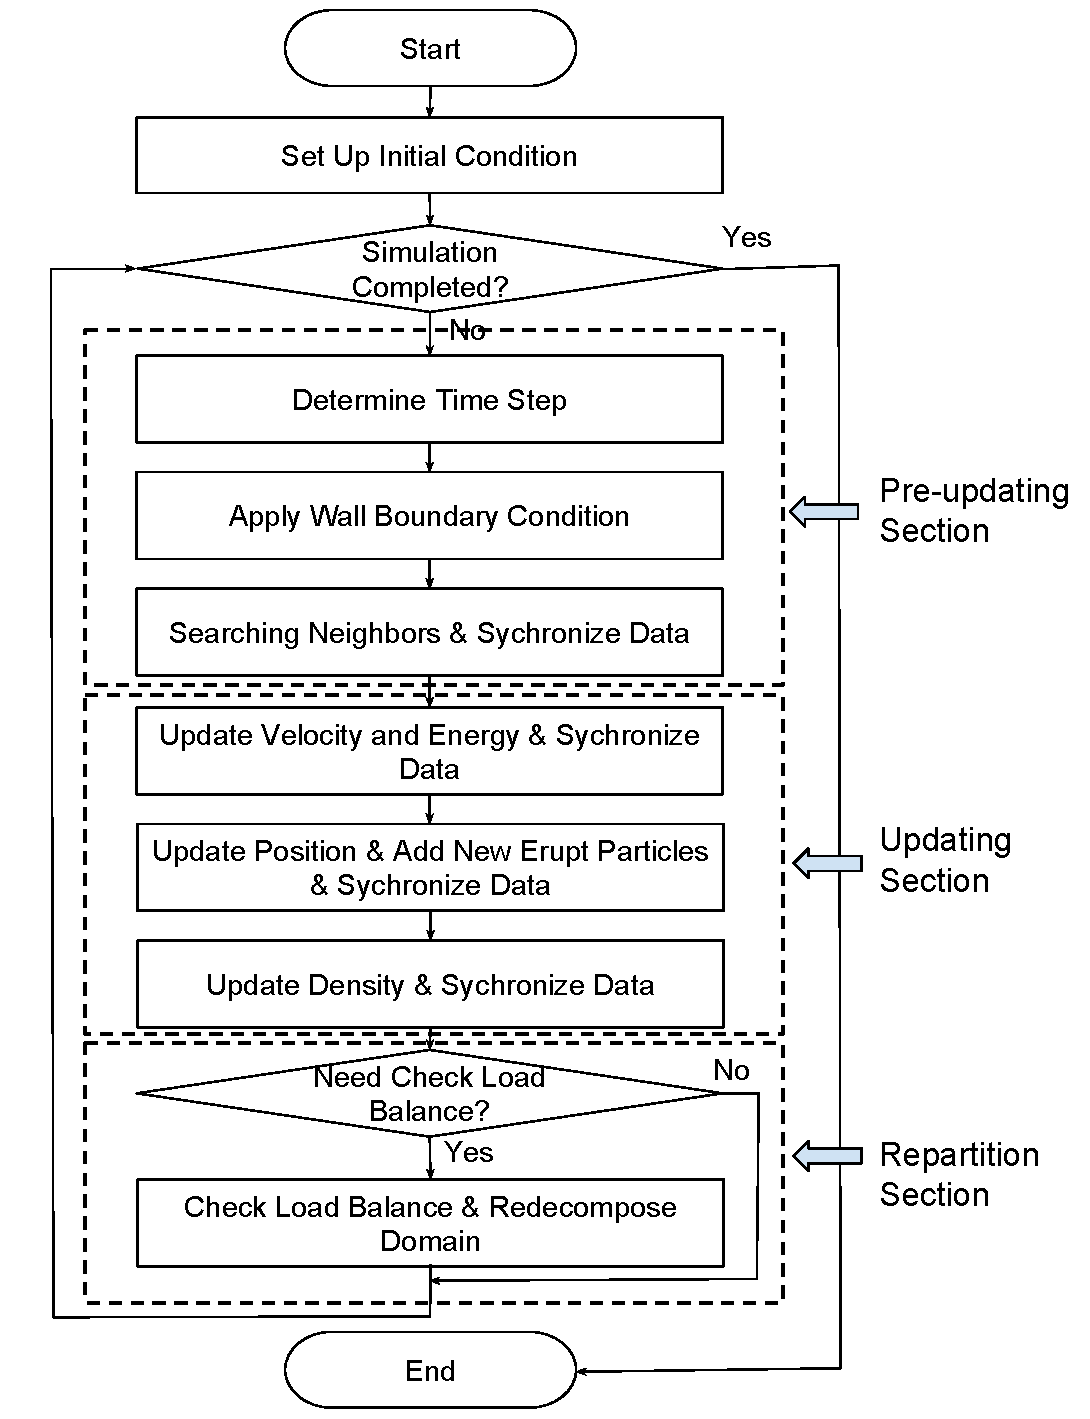
\includegraphics[scale=0.28]{Work_flow}
\hfil
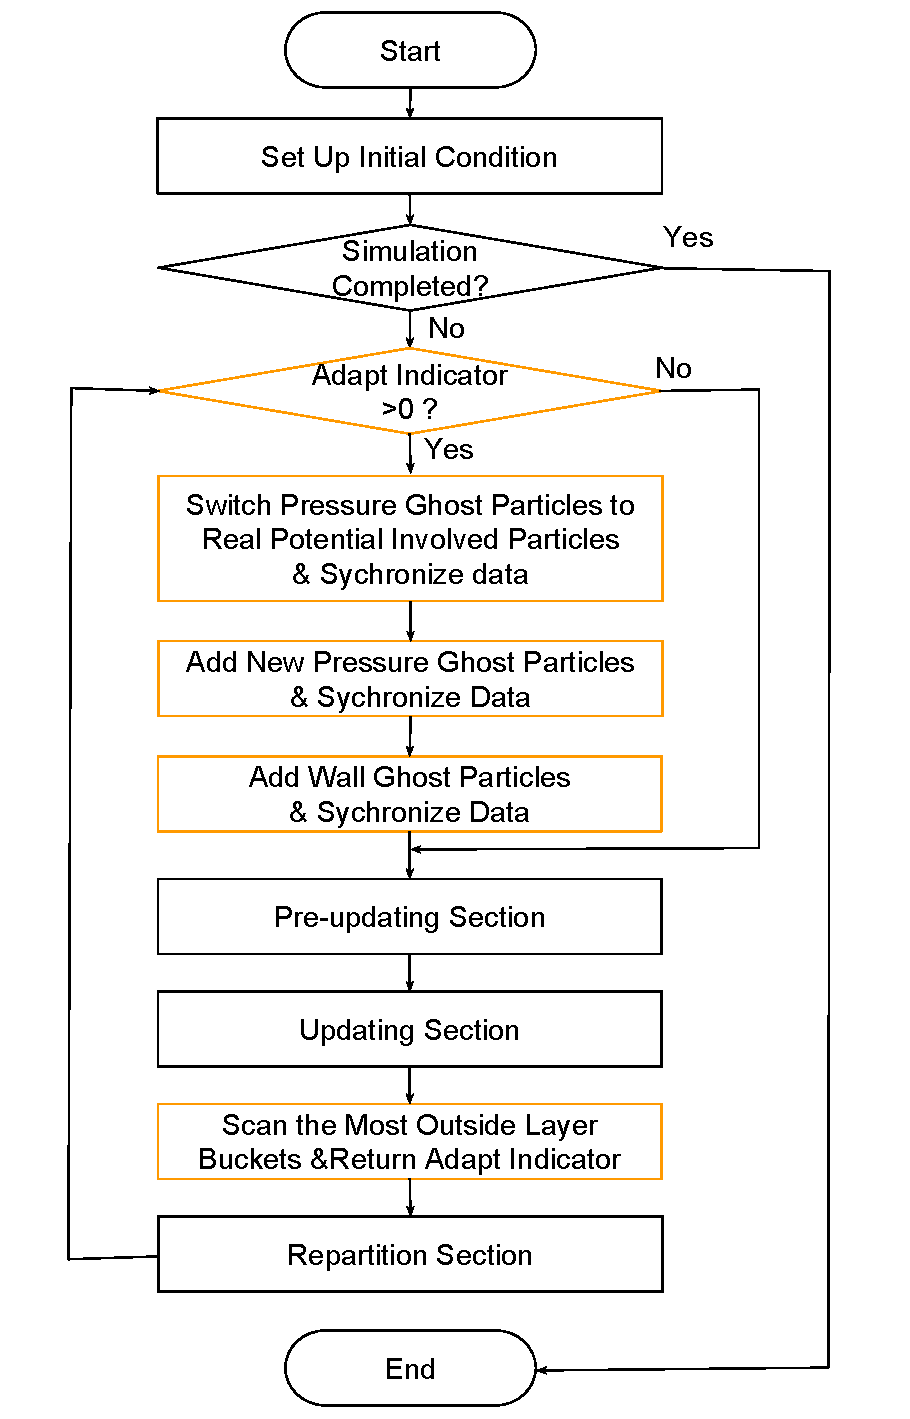
\includegraphics[scale=0.28]{Work_flow_adjust}
\caption{Work flow for SPH code, left is the basic work flow, right is for domain adjusting.}
\label{fig:Work_flow}
\end{figure*}
SPH is a meshfree, Lagrangian method. The domain is discretized by particles and the position of each particle is updated at every time step. The physical laws written in the form of partial differential equations need to be transformed into the Lagrangian particle formalism of SPH. Using a kernel function that provides the weighted estimation of the physical properties in the neighborhood of a discrete point (particle), the integral equations are evaluated as sums over neighbor particles. Only particles located within support of kernel function will interact. Thus, physical properties associated to the particle are updated based on its neighbors. A neighbor searching needs to be carried out before updating of physical properties. A basic work flow of our SPH code is shown in figure \ref{fig:Work_flow}. We use buckets, which contain all particles associated with a sub-domain (see Fig. \ref{fig:SFC_domain_decomposition}) 
and keep stationary during the entire simulation, to reduce searching cost (since search can now be restricted to only neighboring domains).
Domain is decomposed based on a SFC going through centroids of all buckets, as shown in Fig. \ref{fig:SFC_domain_decomposition}.
\subsection{SFC based indexing}
Our data structure starts from assigning each particle and bucket an identifier, we refer to it as key, which should be unique throughout simulation. The key for a bucket is determined by centroid coordinates of the bucket while the key for a particle is determined by adding coordinates and adding time step of the particle. The map from coordinates to key is based on SFC \cite{sagan2012space} which maps a n-dimentional domain to a one dimentional sequence. The standard procedure for obtainning SFC is: 
\begin{itemize}
\item Scale all coordinates into a "box" $[0,1]^n $: $\textbf{X}^\prime \rightarrow \textbf{X}$
\item Compute $k_r = h_n(\textbf{X})$. Where $h_n$ is the map $h_n: [0,1]^n \rightarrow [0,1]$. 
\item Convert $k_r$ to integer $k$ by multiplying $k_r$ with a large integer and removing decimal part.
\item Sort all keys to form a SFC sequence. The SFC represents a curve passing through all particles (or centroids of buckets).
\end{itemize}
%
\begin{figure*}[!t]
\centering
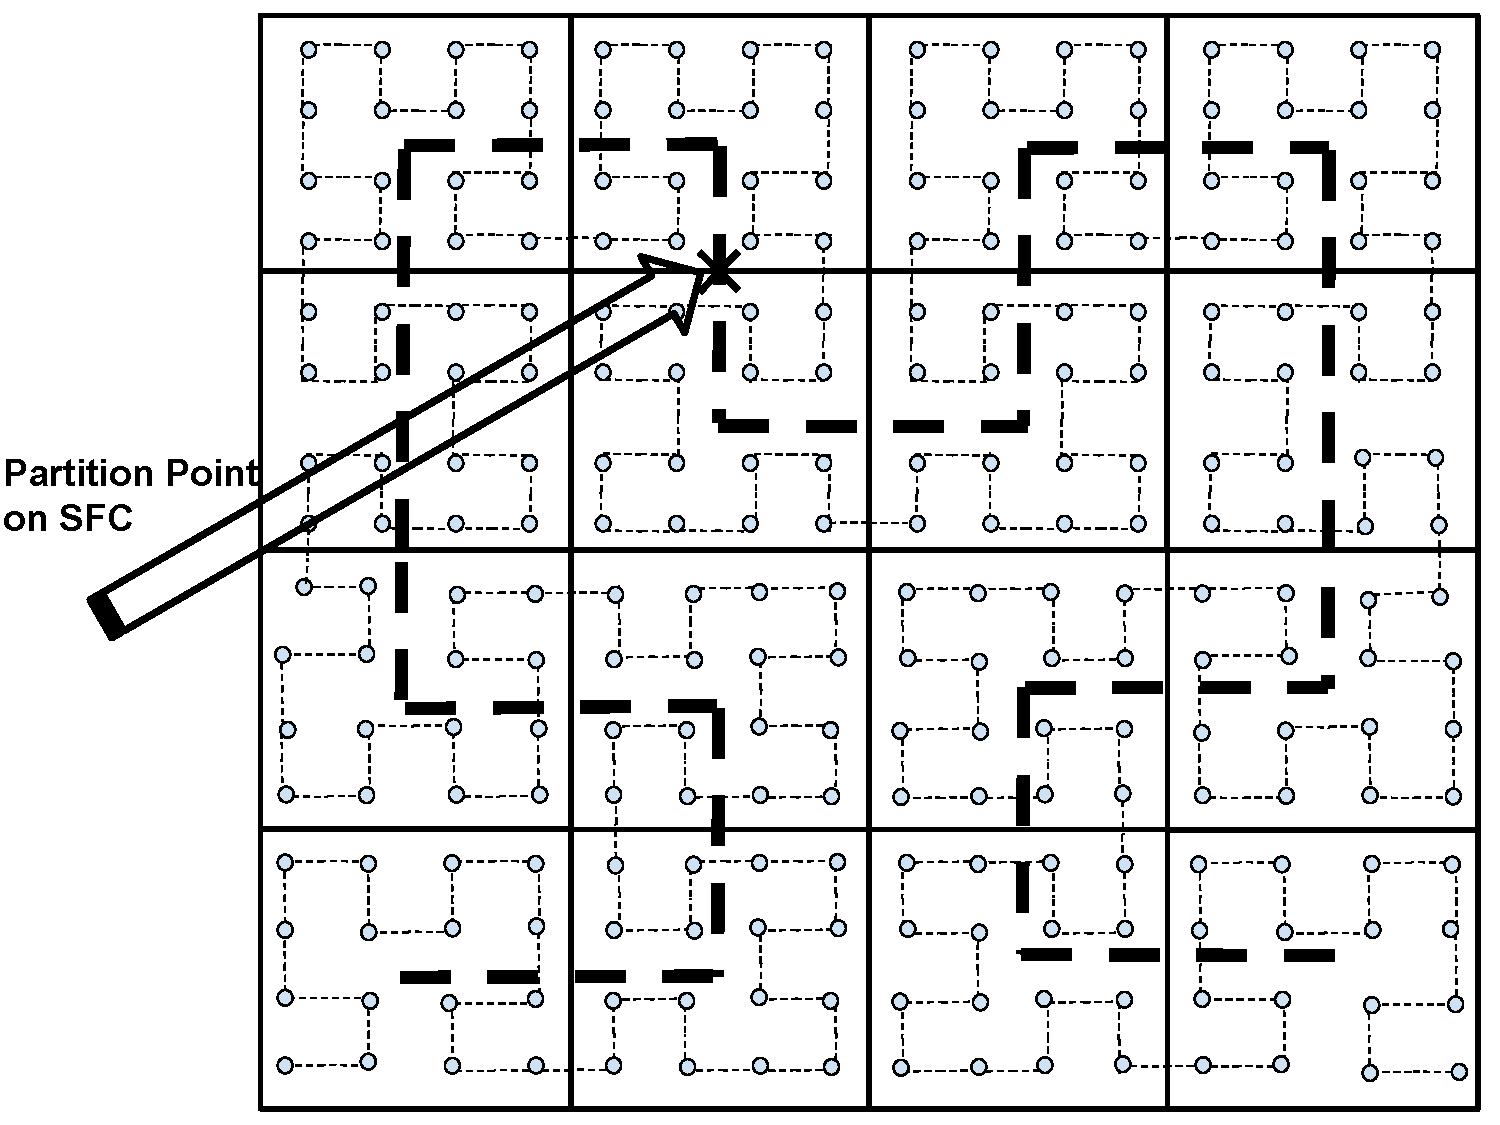
\includegraphics[scale=0.15]{SFC_particles_buckets}
\hfil
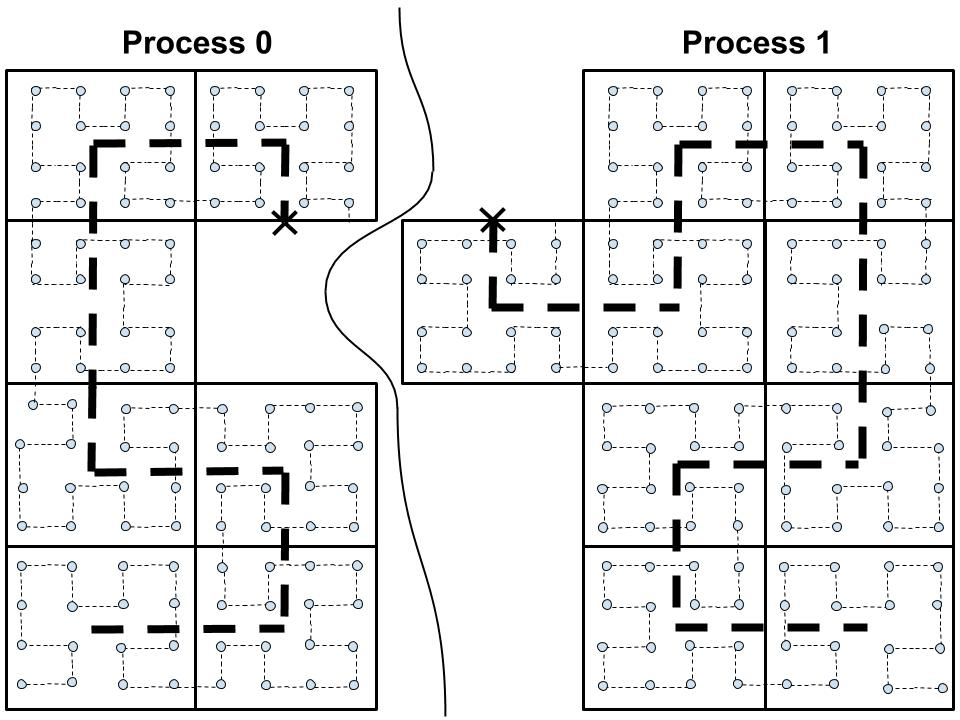
\includegraphics[scale = 0.16]{SFC_particles_buckets_partition}
\caption{The left figure shows SFCs passing all particles and buckets. The right figures shows an example domain decomposition based on SFC of buckets.}
\label{fig:SFC_domain_decomposition}
\end{figure*}
%
Details for constructing the map $h_n$ can be found in \cite{patra1995problem}. These keys denote a simple addressing/ordering scheme for the data, i.e., a simple global index space for all the objects.\\
In some situations, new particles need to be added while simulation. For example, new particles need to be added at the bottom of the eject vent (see figure \ref{fig:Particle_adding_with_link}). To distinguish particles added at the "same position" but at different time steps, we extend the SFC-based key to time-dependent SFC based key by including date of birth of particles into their keys. The time-dependent SFC based key can be denoted as: $[k,t]$, where $t$ is the time step. The map $h_n$ will become:
\begin{equation}
h_n: [0,1]^n \times \textbf{T} \rightarrow [0,1] \times \textbf{N}
\end{equation}
Where $\textbf{T} \subset [0,\infty)$ is the time dimension, and $\textbf{N}=\lbrace 0, 1, 2, 3...\rbrace$.
To guarantee locality, sorting of particle keys is majorly based on $k$, that is to say, particle with smaller $k$ always comes before particles with larger $k$. For these particles have the same $k$, ordering of them will depend on $t$. Figure \ref{fig:SFC_domain_decomposition} shows SFC ordering of buckets and particles in buckets. 
Several features of such indexing scheme are suitable for SPH:
\begin{itemize}
\item Guarantee uniqueness of keys.
\item Key of each object is generated purely based on its own coordinates. When we add new objects on different processes, key of each object can be generated fast and independently.
\item Objects that are located closely in the Euclidian space will also be close to each other in the one dimensional SFC key space in the mean sense. Since SPH particles only interact with its neighbors, geometric locality can be exploited for efficient access of data.
\item This type of key effectively generates a global address space. Globality of key and conservation of locality make it easy to partition the sorted key sequence and obtain a decompositiion of the problem.
\end{itemize}
\subsection{Data management strategies}
%\subsubsection{Particle and bucket}
The most basic data structure of SPH are particles and buckets. Both are defined as C++ classes. Information that is contained in particle class can be categorized into six categories: ID(the key), affiliate(rank of the process that the particle belongs to), primitive variables (variables show up as unknowns in governing equations, e.g. density, velocity), secondary variables (physical properties that can be computed from primitive variables, they are stored to avoid repeated computations eg. pressure, temperature), flags (indicators, such as indicator for ghost particle and real particles) and neighbor information (it is a vector of particle keys in our application). Similarly,  information that is contained in  a bucket class can also be categorized into different categories: ID, affiliate, dimension information (maximum and minimum coordinates, boundary information), flags (indicators, such as indicator for guest and non-guest), neighbor information (keys of 27 neighbor buckets including its own key) and owned particles (it is a vector of particle keys in our application). Objects defined based on these two classes are then accessed through hash tables.\\
%\subsubsection{Hash table and hash conflict}
One of the fundamental data structures that allows flexible data access is a hash table. Based on the keys of data, the address-calculator(hashing) function determines in which slot the data should be stored:
\begin{equation}
slot\,index = hash(key)
\end{equation}
Data in a hash table can be access with time complexity of O(1)) when there is no hash conflicts. One way to handle hash conflicts is to use an additional sorted vector attached to the hash table. When several keys hash to the same slot, a vector will be created. The vector is sorted based on keys so that a binary search (with an average time complexity of O(log n)) can be used to find the correct position for adding, deleting or retrieving of data. Another option is using an additional linked list which is more flexible in memory allocation but slower in searching (O(n)). In addition, pointer based memory accessing of link list will greatly slow down the efficiency of data access for long link list. Choosing of proper way to handle hash conflicts greatly depends on the problem itself. For volcano plume simulation, new particles are added at the bottom of the eruption vent (see Fig. \ref{fig:Particle_adding_with_link}). So the linked list is a better choice for us. Pointers to these new particles will be stored in external linked lists as shown in Fig. \ref{fig:Particle_adding_with_link}.
\begin{figure}
\CenterFloatBoxes
\begin{floatrow}
\ffigbox
{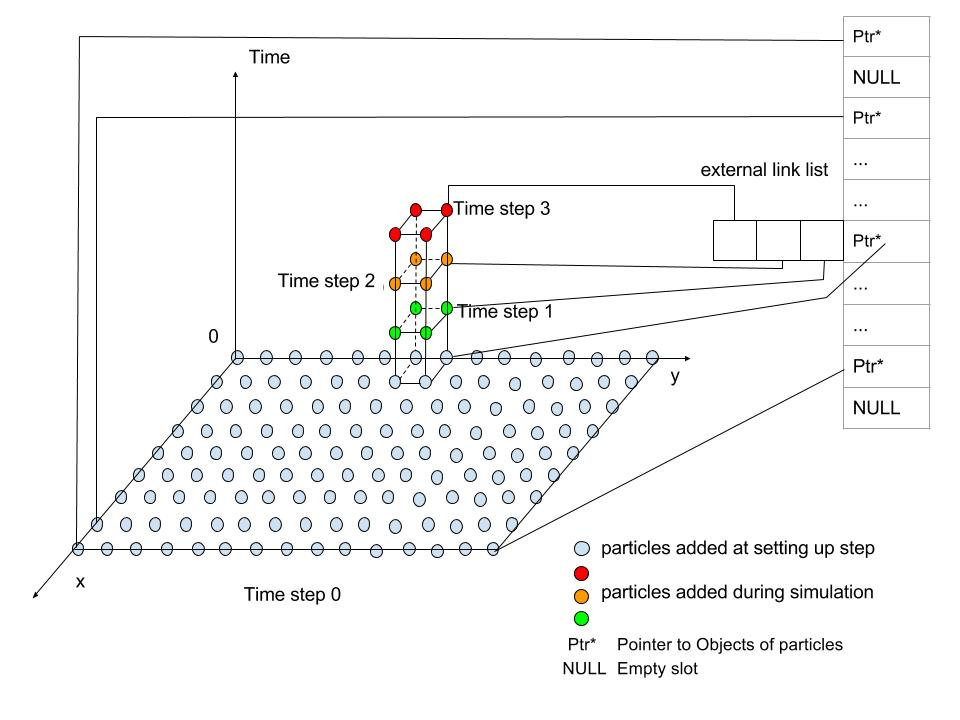
\includegraphics[scale=0.23]{Particle_adding_with_link}}
{\caption{Non-uniform distribution of particles in the $[0,1]^n \times \textbf{T}$ space due to adding of new particles at a small area of the whole domain.}
\label{fig:Particle_adding_with_link}}
\killfloatstyle
\ffigbox
{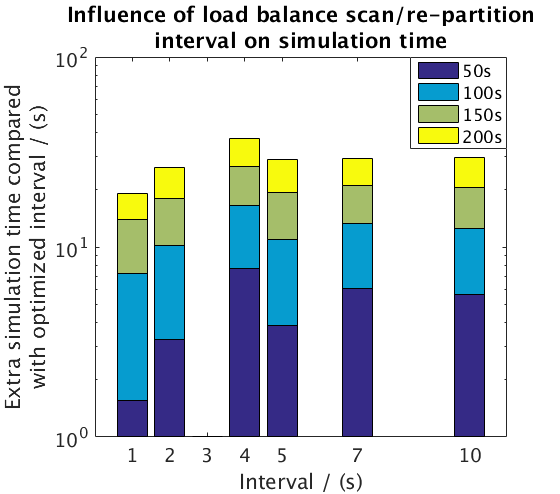
\includegraphics[scale=0.35]{int_bar}}
{\caption{The influence of different load balance check intervals on simulation time. The bar values are the extra simulation time in log scale. The optimized interval is 3s.}
\label{fig:check_int}}
\end{floatrow}
\end{figure}
%\subsubsection{Hash function for time dependent key}
For time-independent keys, the hash function can be a simple function like:
\begin{equation}
Slot\,Index= \frac{Key - Min\,Key}{Max\,Key - Min\,Key} 
\times Hash\,Table\,Size 
\label{eq:hash_function}
\end{equation}
One natural way to hash time-dependent key $[k,t]$ is to convert the two elements in the key into one number taking $k$ as the higher digit and $t$ as the lower digit of the large number. However, for volcano plume simulation, only ghost particles for eruption boundary condition will be successively added at the same place: bottom of the vent. That is to say, particles are distributed non-uniformly in the $[0,1]^n \times \textbf{T}$ space as shown in figure \ref{fig:Particle_adding_with_link}. To avoid non-uniform sparse hash table and conserve locality, we only plug the first number, $k$, of the key, $[k,t]$, into the hashing function, Eq. (\ref{eq:hash_function}). All particles with the same birth location will hash to the same slot and handled by external linked list.
\subsection{Load balancing strategy}
\label{sect:load_balance}
%\subsubsection{Weighted work load} \label{sec:Weighted_work_load}
Particles in our problem can be categorized into four types: real particles, wall ghost particles, pressure ghost particles and eruption ghost particles. Ghost particles are for imposing of corresponding boundary conditions. As different types of particles involve different amount of computational work, shown by table \ref{tab:Computational_cost_steps}, we assign different work load weight for different types of particles based on profilling data. Instead of simply using number of contained particles as work load for buckets, work load of each bucket is determined by summing up work load weights of all particles within the bucket. The SFC of buckets now becomes a weighted sequence. Domain decomposition  is conducted by cutting the weighted SFC of buckets into pieces. Each piece of SFC should have balanced total weights.
\begin{table}[htp]
	\begin{centering}
	\caption{Computational cost per particle for different steps}		
	  \begin{tabular}{lrrrrrr}
	    \hline
	    Step & Cost ($ms$) & Real & wall & eruption & pressure\\
	    \hline
	    neighbor search & 0.41 & Yes & No & No & No \\
	    update momentum and energy & 0.70 & Yes & No & No & No\\
	    update density & 0.42 & Yes & No & No & No \\
	    update position & 0.01 & Yes & No & Yes &  No\\
	    velocity filtering& 0.43 & Yes & No & No & No\\
	    apply wall bc     & 0.75 & No & Yes & No & No\\
	    summation ($ms$) & - & 1.97 & 0.75 & 0.01 & 0.00\\
	    \hline
	  \end{tabular}
	  \label{tab:Computational_cost_steps}	
	\end{centering}
\end{table}
%
%\subsubsection{Domain decomposition and dynamic load balancing}
Figure \ref{fig:SFC_domain_decomposition} shows how domain is decomposed based on partition of SFC of buckets. The particles are automatically split into several groups along with buckets that contain them. As SFC of buckets is a curve in the three dimensional space, partition of this curve will automatically lead to 3D domain decomposition. 
Movement of particles, adding of new particles and adjusting of domain will lead to important load imbalance between processes. To restore load balance, computational load is monitored at a given interval which is optimized based on numerical experiments. Repartitioning is carried out when load imbalance is larger than a given tolerance.
\\
As some of the neighbor particles reside in other partitions. A set of "guest" particles and buckets are used to synchronize data across partitions. To minimize communications, data is synchronized only where needed, using non-blocking MPI communications. 
\section{Adjusting of Domain During Simulation} 
For plume simulation and many similar/related phenomena, where some fluid ejects into stationary fluid and gets mixed, the stationary fluid must be represented.
A lot of CPU time will be spent on computing associated with these stationary particles. If simulating of stationary particles can be avoided, the computational cost will be reduced greatly.
We propose a simple strategy to add such feature in our code with low computational cost. We add a scan function to monitor the outermost layer of the domain. When the ejected fluid reaches the boundary of the current domain, pressure ghost particles will be turn to real particles and then add a new layer of pressure ghost particles for pressure boundary conditions. The original work flow is modified to enable such a feature (see Fig. \ref{fig:Work_flow}).\\
A involved-flag is added to particle class to distinguish different states of involvement. Particles are categorized into three groups based on the value of the involved-flag: involved, potentially involved, and not involved. The involved particles are particles that have already been affected by the mixing. The potentially involved particles are particles that have not been involved in mixing but are adjacent to involved particles and will thus be involved in the near future. 
All communication and computation associated with uninvolved particles can be ignored. That is to say, only potential involved and involved particles need to be simulated.
As simulation progresses, the ejected fluid will reach larger area and more and more particles will be influenced. When originally stationary air is influenced by erupted material, the mass fraction of the erupted material will increase from zero to a positive value. So we can determine whether a particle should turn to involved based on whether the mass fraction of that particle is larger than a given threshold ($10^{-5} $ in our simulation) or not. Other physical properties, like velocity, can also serve as alternative "switching criteria".\\
A similar scheme is also deployed for buckets resulting in a categorization of buckets. The additional complexity is that potentially involved ghost particles must also be accounted for.
\begin{figure*}[!t]
\centering
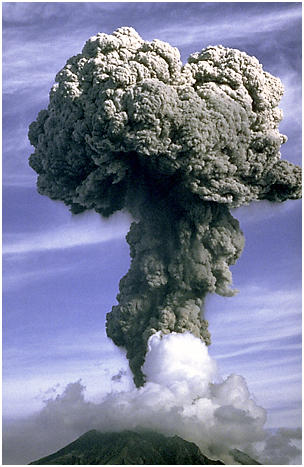
\includegraphics[width=3.8cm,height=4.0cm]{plume_photo}
\hfil
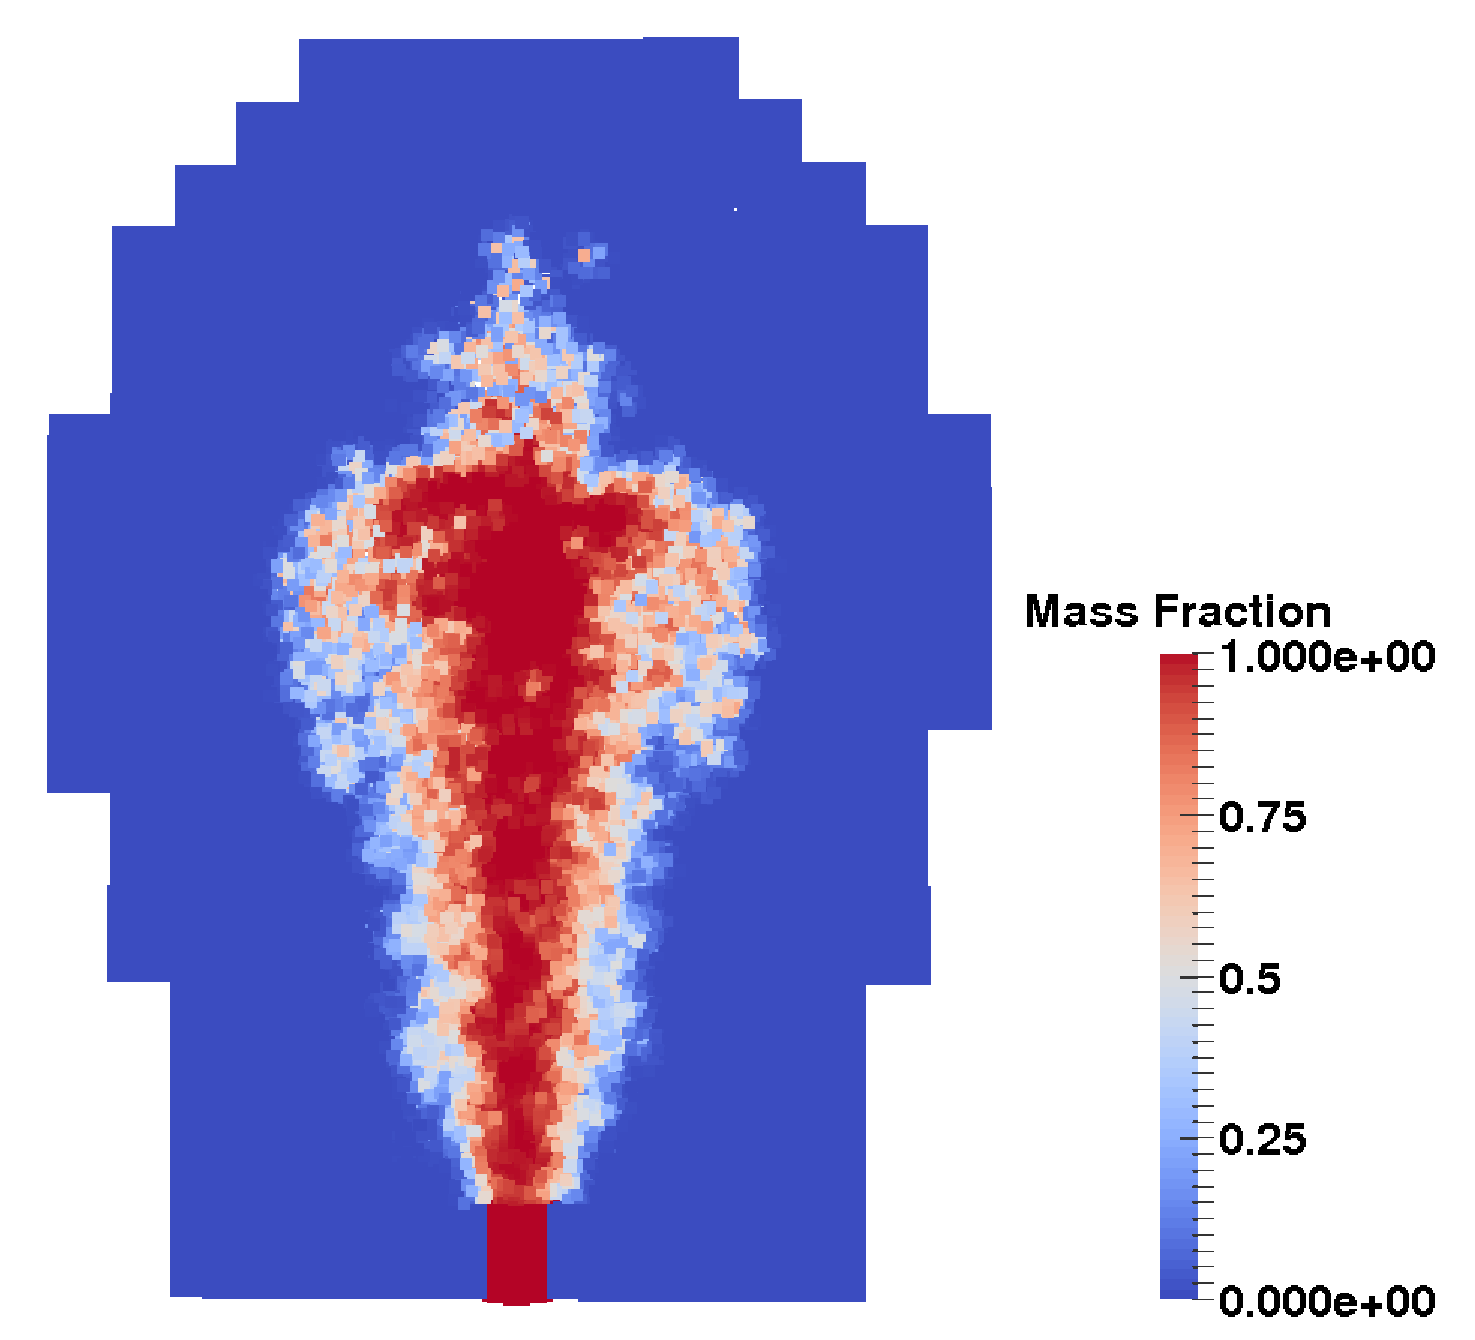
\includegraphics[width=3.8cm,height=4.0cm]{Plume_simulation}
\caption{Left figure shows plume from Sakurajima Volcano eruption\cite{PlumePhoto}, right figure shows a typical simulation results with the same input parameters of "Run P1" in reference \cite{suzuki2005numerical}.}
\label{fig:Plume}
\end{figure*}
\section{Numerical Test}
We use the same governing equations, boundary conditions and input parameters as the model developed by Suzuki \cite{suzuki2005numerical}. %Details about discretization of the governing equations will not be covered in this paper, neither. 
A typical simulation result of volcano plume by our code is shown in Fig. \ref{fig:Plume}.
%
\subsection{Scalability test}
\begin{figure*}[!t]
\centering
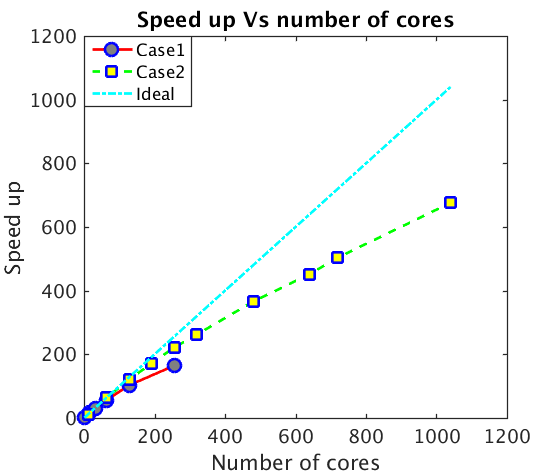
\includegraphics[scale=0.31]{strong_scale}
\hfil
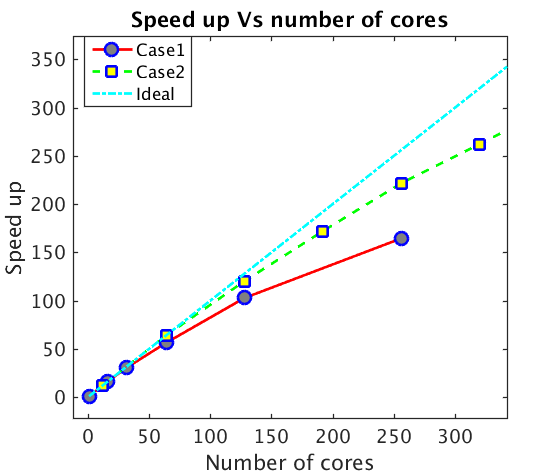
\includegraphics[scale=0.31]{strong_scale_zoom}
\hfil
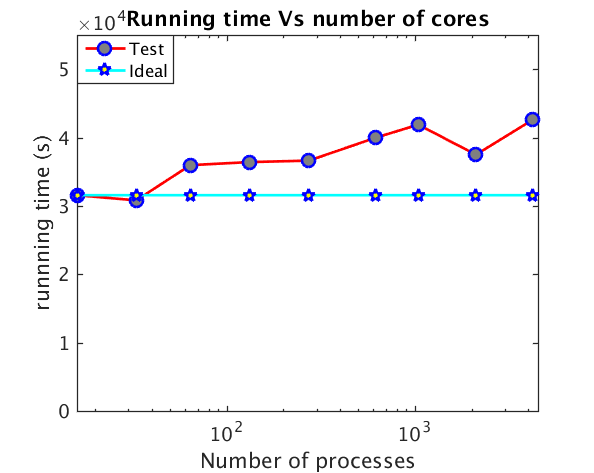
\includegraphics[scale=0.31]{weak_scale}
\caption{The first figure shows strong scalability tests result. middle figure is the zoomed view of first one. It is obviously shown that strong scalability is better when problem size is larger. The third figure is weak scalability test results}
\label{fig:2cases_efficiency}
\end{figure*}
%
Experiments have been carried out on the computational cluster of Center for Computational Research (CCR) at Buffalo. 
The processors are 12 cores E5645 running at 2.40GHz clock rate with 4GB memory per core on a Q-Logic Infiniband network. Each node comprise of two sockets with several of these processors. Memory and level 3 cache are shared on each node. The simulational domain is a box with initial dimension $[-4.8km, 4.8km]\times [-4.8km, 4.8km] \times [0km, 6km]$ for case 1 and $[-10km, 10km]\times [-10km, 10km] \times [0km, 5km]$ for case 2. The smoothing length (we set initial intervals between particles equal to smoothing length) equals to 200m and 100m respectively for test case 1 and test case 2. So the computational work load of test case 2 is larger than that of the test case 1. The simulations run for 20s physical time.  Parallel speed up are shown in Fig. \ref{fig:2cases_efficiency}. Test case2 shows better speed up than test case1 which implies that the overhead of strong scalability can be increased by increasing total amount of work load.
The weak scalability test is conducted with the same initial domain as test case 1 and various smoothing length. Each simulation runs for 400 time steps. The average number of real particles of each process keeps constant at $25900$, so the average work load for each processor are keep constant. 
As shown in figure \ref{fig:2cases_efficiency}, simulation time are almost constant with some minor fluctutations.\\
\subsection{Effect of workload check interval calibrated particle weight}
\begin{table}[htp]
	\begin{centering}
      \caption{Simulation time for same particle weight and different particle weights }		
	  \begin{tabular}{lrrrr}
	    \hline
	    Physics time & 10 s & 20s & 30 s & 40 s \\
	    \hline
	    Same weight & 1141.7 & 4119.4 & 10371.0 & 12453.7\\
	    Different weight & 1108.2 & 4057.0 & 10281.5 & 12166.3\\
	    \hline
	  \end{tabular}
	  \label{tab:same_diff_particle_weight}
	\end{centering}
\end{table}
In section \ref{sect:load_balance}, we proposed to use different particle weight for different types of particles when estimate the weight of buckets. The effect of using different particle weight is demonstrated in table \ref{tab:same_diff_particle_weight}. The simulation time is reduced by using different particle weights. However, the amount of time that is reduced is not as significant as our expectation. One possible explanation is that real particles are the major population, so the load imbalance caused by assignning improper weight value to ghost particles is small.\\
The best load balance check interval is calibrated based on a series of simulations with different load balance scan/repartition intervals. From 0 - 50 seconds, the interval of 1 second shows a better load balance than interval of 2 seconds. However, for the simulation of 50 - 100 seconds, interval of 2 seconds is better. This implies that lose of load balance is faster and requires a more frequent re-decomposition of domain at the initial stage of simulation. This is consistent with the plume development process: the domain grows quickly at beginning as erupted material ejects into the environment and spreads quickly. Afterwards, the spreading speed of the front edge slows down due to viscosity and momentum exchange leading to slowing down of domain growth. We need to emphasize that, these optimized parameters, including weight of particles and load blance checking interval, are case sensitive and need to be re-calibrated for different applications and hardware architecture.
%
\subsection{Domain adjusting}
\begin{figure}
\CenterFloatBoxes
\begin{floatrow}
\ttabbox
{	  
    \begin{tabular}{lrr}
    \hline
    Functions & Total time (s) & Called times\\
    	\hline
    UPME & 2954.8 & 201 \\
    UPP & 38.55 &  201 \\
    ADPP & 21.51 & 3 \\
    ADWP  & 8.88 & 3 \\
    SWCH & 0.08 &  2 \\
    SCN  & 7.72 & 201 \\
    \hline
  \end{tabular}
}
{\caption{Computational work load of extra steps for domain adjusting. SWCH represents step that switch pressure ghost particle to real particle, ADPP is short for adding new pressure ghost particles, ADWP represents adding wall ghost particles step, SCN is short for scanning the most outside layer of the domain.}
\label{tab:Computational_cost_doamin_adj}}
\killfloatstyle
\ffigbox
{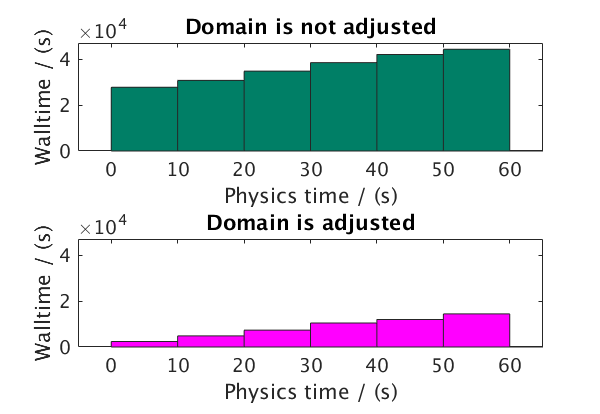
\includegraphics[scale=0.35]{adj_vs_no}}
{\caption{The figure on the top shows simulation time without domain adjusting, the figure on the bottom shows simulation time with domain adjusting. Different bins represent simulation time up to specific physics time indicated by $x$ axis.}
\label{fig:adj_vs_no}}
\end{floatrow}
\end{figure}
For the test problem in this paper, the volcanic plume will finally reach to a region of $[-10km \,\,\, 10km] \times [-10km\,\,\,10km] \times [0km\,\,\,20km]$ after around 300 seconds of eruption. When numerical simulation goes up to 90 seconds, the plume is still within a region of $[-3km\,\,\,3km] \times [-3km\,\,\,3km] \times [0km\,\,\,6km]$. This implies that adjusting of domain can avoid computing large number of uninfluenced air particles, especially for the beginning stage of simulation. On the other hand, additional functions (see Fig. \ref{fig:Work_flow}) for domain adjusting will add extra computational cost. Table \ref{tab:Computational_cost_doamin_adj} shows the extra computational cost corresponding to these functions. Profilling data for momentum and energy update (UPME) and position update (UPP) is also included in the table for the purpose of comparison. As we can see from the table, the cost of SCN is even smaller than UPP fucntion, which is the cheapest function (as shown in table \ref{tab:Computational_cost_steps}) in the regular framework (see Fig. \ref{fig:Work_flow}). Other three functions, ADPP, ADWP and SWCH, only called fewer times during the simulation, and as a consequence, the extra computational cost due to them are neglectable. To summarize, the additional cost caused by domain adjusting functions is ignorable.
Figure \ref{fig:adj_vs_no} shows that simulation time of the test problem is greatly reduced when we adopt the domain adjusting strategy in our code.
\section{Conclusion}
We developed data management strategies for parallel implementation of SPH method using MPI standard to simulate volcano plume. Neighbors searching and domain decomposition is based on background grid. SFC based index scheme is adopted to identify buckets and time-dependent SFC keys are  used as identifier for particles. 
Hash tables with external link list are adopted for accessing particles and buckets data. Based on calibrated particle work load, a dynamic load balance strategy is developed by checking load balance and redecomposing the domain at an optimized interval. The performance of the code was further improved to several times faster by adjusting computational domain during simulation. 
A overall good scalability and performance improving is obtained.\\
The flexibility of data accessing enables implementing of meshless methods for solving of more complicated problems and using of more advanced techniques, such as dynamic particle splitting techniques\cite{vacondio2012accurate, feldman2007dynamic}, which will give higher resolution at the area of interest by splitting one large particle to several smaller ones. The data structure, particle and bucket indexing strategies, domain decomposition, dynamic load balancing method and domain adjusting strategies in this paper can be adopted by other implementations of any meshfree methods (include SPH).
%------------------------------------------------------------------------------
% Refs:
%
\label{sect:bib}
\bibliographystyle{plain}
%\bibliographystyle{alpha}
%\bibliographystyle{unsrt}
%\bibliographystyle{abbrv}
\bibliography{Reference}

%------------------------------------------------------------------------------


%------------------------------------------------------------------------------
% Index
%\printindex

%------------------------------------------------------------------------------
\end{document}

% EOF
